\documentclass[10pt,twocolumn]{article}

\usepackage[margin=0.72in]{geometry}
\usepackage{amsmath,amssymb}
\usepackage{booktabs}
\usepackage{graphicx}
\usepackage{url}
\usepackage{xcolor}
\usepackage{caption}

\graphicspath{{report_figures/}}
\setlength{\columnsep}{0.24in}
\captionsetup{font=small,labelfont=bf}

\title{\textbf{Standard Deep Ensembles versus Concrete Dropout}\\
\large Predictive Accuracy and Uncertainty for Gaussian Regression}
\author{Your Name \quad\texttt{CS 6956}}
\date{\today}

\begin{document}
\maketitle

\begin{abstract}
This report compares standard deep ensembles with Concrete Dropout for
heteroscedastic regression.  Each standard ensemble member is independently
initialized and trained with an explicit $L_2$ penalty, corresponding to a
zero-mean Gaussian weight prior.  Concrete Dropout instead learns dropout
probabilities and uses stochastic forward passes from one fitted network.
Experiments use a two-dimensional synthetic problem with known nonlinear mean
and input-dependent noise, followed by the ten-feature scikit-learn diabetes
data set.  On the synthetic data, standard ensembles have slightly lower
error and narrower intervals, while Concrete Dropout gives closer-to-nominal
90\% coverage and substantially larger epistemic uncertainty.  On diabetes,
the two methods have similar test NLL and RMSE, but Concrete Dropout remains
more conservative in its intervals.  These results illustrate that matching
the number of predictive components does not make independently trained
networks and dropout masks equivalent sources of uncertainty.
\end{abstract}

\section{Introduction}
Deep neural networks can achieve good point-prediction accuracy while
remaining overconfident away from the training distribution.  Predictive
uncertainty is useful both for identifying difficult examples and for
distinguishing observation noise from uncertainty about the model itself.
This work studies two practical approximate Bayesian strategies.  A standard
deep ensemble trains multiple networks from different random initializations
and random seeds \cite{lakshminarayanan2017}.  Concrete Dropout learns
continuous dropout probabilities, allowing dropout to remain stochastic at
test time \cite{gal2017concrete}.

The central question is: \emph{when the number of predictive components is
matched, how do the methods differ in accuracy, calibration, and the
aleatoric/epistemic decomposition?}  The experiment first uses a synthetic
two-dimensional regression task, where the data-generating function and noise
are known.  It then evaluates the methods on a higher-dimensional,
realistic regression problem.  Both training and held-out test performance
are reported.

\section{Methods}
\subsection{Probabilistic regression model}
Every network is a two-hidden-layer ReLU MLP with 64 units per layer.  Its
output is a mean and log variance,
\[
 p(y\mid x,W)=\mathcal{N}\!\left(y;\mu_W(x),\sigma_W^2(x)\right),
\]
trained with Gaussian negative log likelihood (NLL).  The predicted
observation variance is interpreted as aleatoric uncertainty.  Variation in
the predicted means across members or stochastic passes is interpreted as
epistemic uncertainty.

For a standard ensemble of $S$ members, the objective is
\[
 \mathcal{L}_{\rm DE} =
 \frac{1}{n}\sum_i {\rm NLL}(y_i\mid x_i,W)
 +\lambda\sum_l\lVert W_l\rVert_2^2,\qquad
 \lambda=10^{-4}.
\]
The second term is the negative-log-prior contribution of an isotropic
Gaussian prior on the weights, up to a constant and scale convention.
Members use distinct seeds and are trained independently.

Concrete Dropout replaces ordinary dropout with a differentiable relaxed
Bernoulli mask and learns a dropout probability $p_l$ for each hidden layer
\cite{gal2017concrete}.  Its regularizer contains a scaled weight-prior term
and the dropout entropy term
\[
 \sum_l d_l\left[p_l\log p_l+(1-p_l)\log(1-p_l)\right],
\]
with entropy coefficient $10^{-3}$.  At evaluation time, the same network is
run with stochastic masks.  Thus, a comparison with $S$ standard members
uses $S$ Concrete Monte Carlo passes, but these components are correlated
draws from one learned model rather than independently trained models.

For component means $\mu_s$ and variances $v_s$, predictions are aggregated
using the law of total variance:
\[
 \bar\mu=\frac{1}{S}\sum_s\mu_s,\quad
 v_{\rm alea}=\frac{1}{S}\sum_s v_s,\quad
 v_{\rm epi}=\operatorname{Var}_s(\mu_s),\quad
 v_{\rm total}=v_{\rm alea}+v_{\rm epi}.
\]
Mixture NLL is evaluated with log-sum-exp over the component Gaussians.
Nominal 90\% intervals are estimated by sampling the Gaussian mixture, not
by replacing it with a single Gaussian.

\subsection{Data and protocol}
The synthetic data contain 1,500 points uniformly sampled from
$[-2,2]^2$.  The noiseless mean is
\[
 f(x)=1.3\sin(1.5x_1)+0.45x_2^2+0.3x_1x_2,
\]
and the standard deviation increases with both $x_1$ and $|x_2|$:
\[
 \sigma(x)=0.18+0.13\frac{x_1+2}{4}+0.12\frac{|x_2|}{2}.
\]
The fixed split contains 1,125 training and 375 test points.  An OOD grid
from $[-3,3]^2$ is used only for visualization.  The realistic data are
the 442-observation, ten-feature diabetes regression data set from
scikit-learn, split into 331 training and 111 test points.  Predictors and
targets are standardized using training statistics; errors and interval
widths are transformed back to original target units.

The full run trains ten standard members with seeds
\{11,23,37,51,71,83,97,109,127,139\}.  The Concrete model uses seed 11.
Synthetic models are trained for 1,000 epochs and diabetes models for 20
epochs.  Ensemble sizes from one through ten are evaluated.  The main
matched comparison uses $M$ standard members versus $M$ Concrete passes.

\section{Results}
\subsection{Synthetic two-dimensional task}
Figure~\ref{fig:data} shows the noisy training observations.  The known
smooth mean and heteroscedastic noise make this a useful sanity check:
uncertainty should increase where the observation noise is larger, and
epistemic uncertainty should be more visible outside the square used for
training.

\begin{figure}[t]
  \centering
  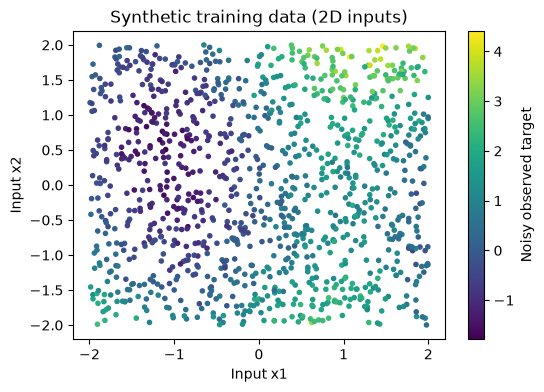
\includegraphics[width=\linewidth]{figure_01.png}
  \caption{Synthetic training data.  The two inputs are sufficient to
  visualize the full input space.}
  \label{fig:data}
\end{figure}

The final per-model standardized test NLLs for the ten standard members range
from 0.021 to 0.066, whereas Concrete Dropout obtains 0.085.  The standard
ensemble's best aggregate test NLL is 0.008 at epoch 50; the Concrete model's
best is 0.026 at epoch 916 (Figure~\ref{fig:learning}).  This early
standard-ensemble optimum is important: continuing to 1,000 epochs gives
excellent fits but does not improve the aggregate held-out NLL.

\begin{figure}[t]
  \centering
  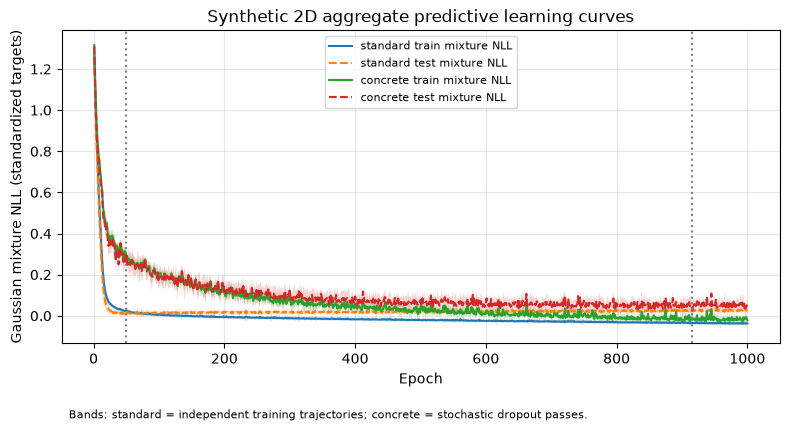
\includegraphics[width=\linewidth]{figure_02.png}
  \caption{Synthetic aggregate predictive learning curves.  Solid and dashed
  lines denote train and test mixture NLL, respectively.}
  \label{fig:learning}
\end{figure}

Table~\ref{tab:synth} reports representative one- and five-component
comparisons.  A single standard member has test RMSE 0.305 and 90\% coverage
0.891.  Five members leave RMSE nearly unchanged at 0.305, slightly reduce
NLL to 0.235, and produce epistemic standard deviation 0.034.  Concrete
Dropout with five passes has test RMSE 0.306, NLL 0.241, coverage 0.915, and
epistemic standard deviation 0.074.  Hence, Concrete Dropout is closer to the
nominal coverage target in this run, but its intervals are wider (1.037
versus 0.963 for standard ensembles).  The extra width comes primarily from
both larger aleatoric estimates and larger stochastic mean variation.

\begin{table}[t]
\centering
\caption{Synthetic test metrics in original target units.}
\label{tab:synth}
\small
\begin{tabular}{lrrrrrr}
\toprule
Method & $S$ & RMSE & NLL & Cov. & Width & SD$_e$\\
\midrule
Standard & 1 & .305 & .239 & .891 & .970 & .000\\
Concrete & 1 & .310 & .251 & .899 & 1.016 & .000\\
Standard & 5 & .305 & .235 & .877 & .963 & .034\\
Concrete & 5 & .306 & .241 & .915 & 1.037 & .074\\
\bottomrule
\end{tabular}
\end{table}

Increasing standard ensemble size changes little after three members: test
RMSE remains approximately 0.304--0.305 and epistemic SD rises from 0.016
at two members to 0.038 at nine members.  This is not a claim that the
uncertainty estimate is monotonically converged; it reflects finite-sample
estimation of member disagreement.  Concrete MC passes improve the one-pass
test NLL from 0.251 to 0.237 at two passes, then stabilize around
0.238--0.241.  Epistemic SD rises from zero by construction to approximately
0.07--0.08.

\begin{figure}[t]
  \centering
  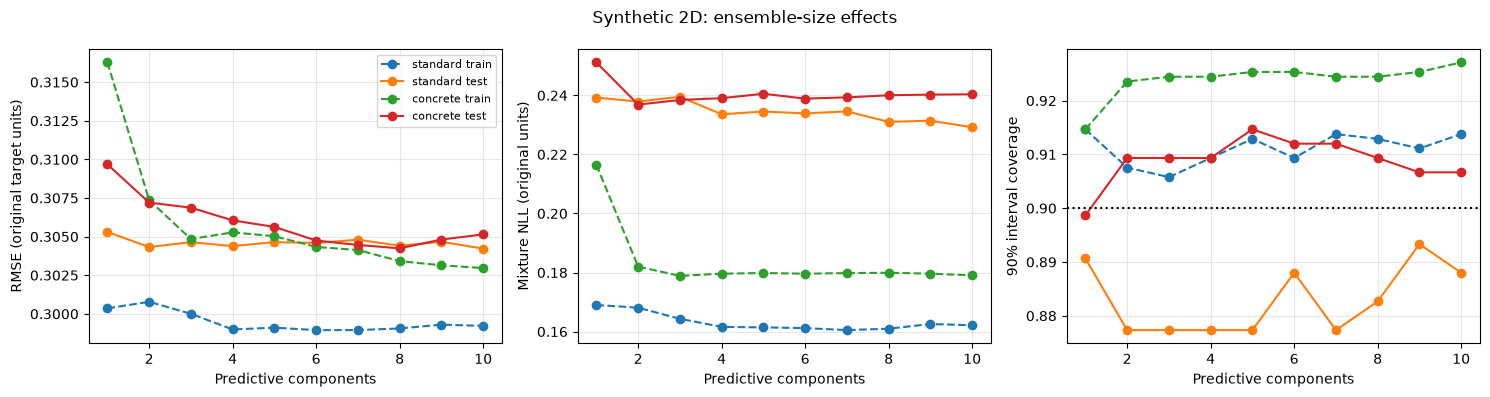
\includegraphics[width=\linewidth]{figure_03.png}
  \caption{Synthetic RMSE, NLL, and 90\% coverage as the matched number of
  predictive components increases.}
  \label{fig:size}
\end{figure}

\subsection{Training versus test behavior and OOD uncertainty}
Training metrics are better than test metrics for both methods.  For example,
the one-member standard model has train/test RMSE 0.300/0.305 and NLL
0.169/0.239.  The five-member Concrete result has train/test RMSE
0.305/0.306 and NLL 0.180/0.241.  The gap is modest on this smooth,
well-sampled problem, but it is visible in likelihood and coverage.

The one-dimensional slice in Figure~\ref{fig:slice} follows $x_2=0$ and
shows that both methods recover the mean function in the training domain.
The OOD maps in Figure~\ref{fig:ood} visualize epistemic standard deviation
outside $[-2,2]^2$.  Concrete Dropout produces stronger and more spatially
diffuse disagreement.  This is useful as an uncertainty signal, but it is
not a guarantee of calibrated OOD probabilities: the OOD grid is synthetic
and was not used to fit or tune either model.

\begin{figure*}[t]
  \centering
  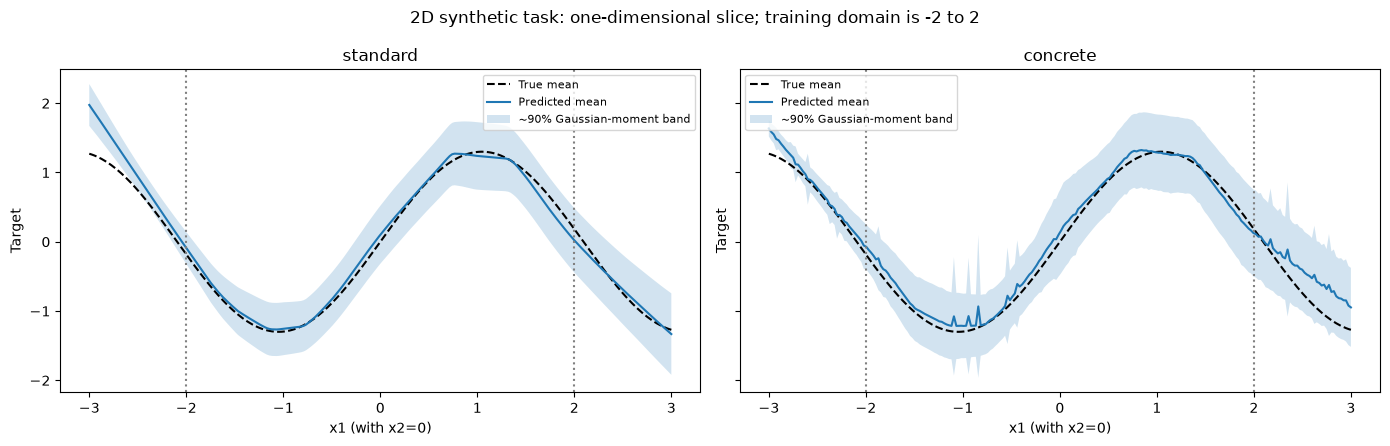
\includegraphics[width=.72\textwidth]{figure_04.png}
  \caption{Predicted means and approximate 90\% moment bands along $x_2=0$.
  Vertical dotted lines mark the training-domain boundary.}
  \label{fig:slice}
\end{figure*}

\begin{figure*}[t]
  \centering
  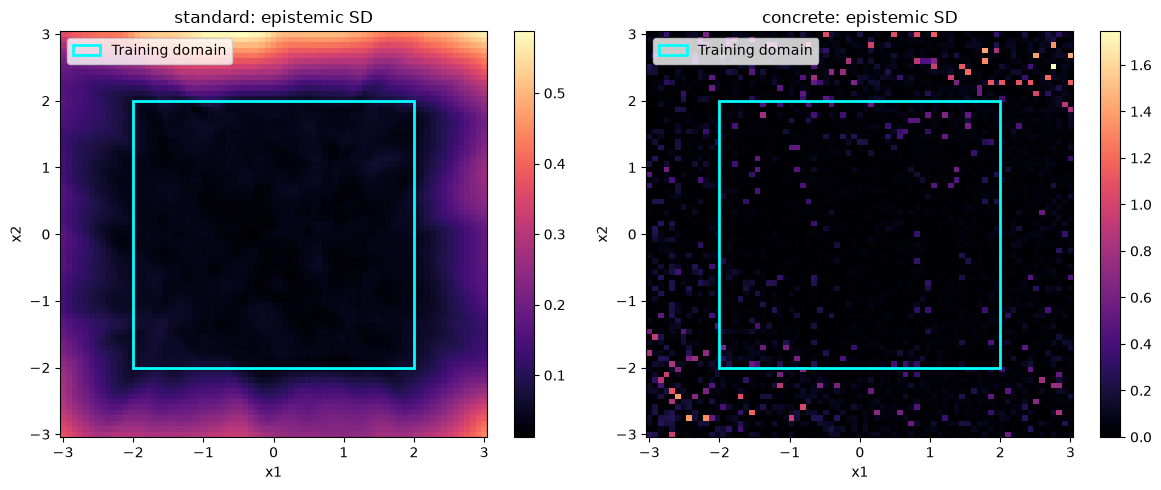
\includegraphics[width=.72\textwidth]{figure_05.png}
  \caption{Epistemic standard deviation over the synthetic input plane.
  The cyan square is the training domain.}
  \label{fig:ood}
\end{figure*}

\subsection{Diabetes regression}
The diabetes task is more data-limited and has ten correlated predictors.
Standard members finish with test NLLs from 1.031 to 1.114 (standardized
target units), while Concrete Dropout finishes at 1.052.  The best aggregate
test NLLs are 1.041 for standard ensembling and 1.022 for Concrete Dropout,
at epochs 13 and 14, respectively.  Thus, the method ranking changes
slightly relative to the synthetic experiment when the model must infer a
ten-dimensional relationship from only 331 training examples.

At five predictive components, standard ensembling gives test RMSE 54.423,
NLL 5.392, coverage 0.883, interval width 159.355, and epistemic SD 7.045.
Concrete Dropout gives RMSE 53.501, NLL 5.354, coverage 0.901, width 171.145,
and epistemic SD 12.873.  Concrete Dropout therefore has the best of these
point and likelihood metrics in this particular split and is closer to 90\%
coverage, at the cost of wider intervals.  The learned dropout rates are
approximately 0.098 and 0.103, compared with 0.0037 and 0.0044 on the
synthetic task.  The difference suggests that the learned regularization
responded to the much smaller, noisier effective data set, although more
seeds and repeated splits would be needed to establish that conclusion.

\begin{figure}[t]
  \centering
  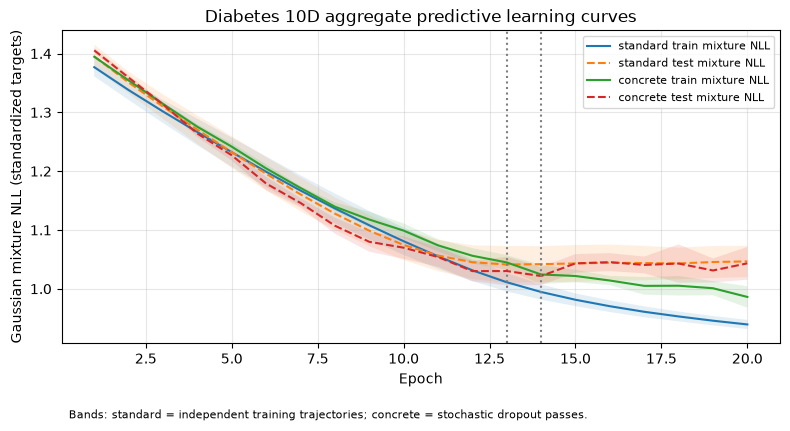
\includegraphics[width=\linewidth]{figure_07.png}
  \caption{Diabetes aggregate predictive learning curves.}
  \label{fig:diabetes-learning}
\end{figure}

\begin{figure}[t]
  \centering
  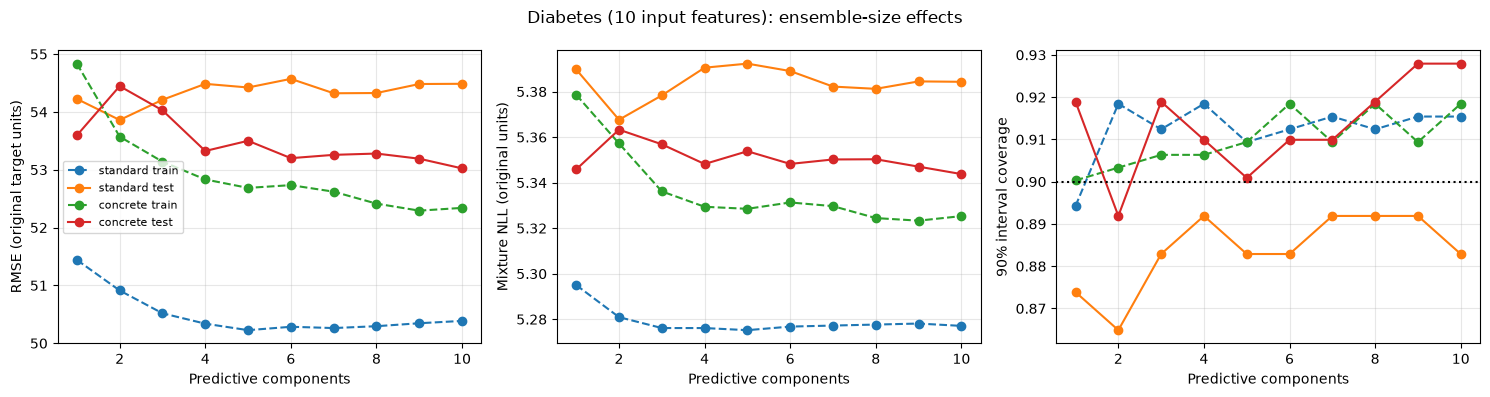
\includegraphics[width=\linewidth]{figure_08.png}
  \caption{Diabetes RMSE, NLL, and 90\% coverage versus predictive
  component count.}
  \label{fig:diabetes-size}
\end{figure}

\section{Discussion and limitations}
The experiments support three conclusions.  First, standard deep ensembles
are a strong accuracy baseline: independent optimization gives low synthetic
error and narrow intervals without requiring learned dropout rates.  Second,
Concrete Dropout produces more epistemic variation and, in these runs,
coverage nearer the nominal 90\% level.  This advantage is not free; the
intervals are wider and the one-network stochastic samples are not equivalent
to independent posterior samples.  Third, the realistic-data ranking is
less decisive.  Concrete Dropout slightly improves the reported diabetes
test metrics, but the data set is small enough that a single split and ten
seeds do not support a broad claim of superiority.

The MC-pass experiment (Figure~\ref{fig:mc}) separates the effect of sampling
from the effect of fitting additional networks.  On the synthetic test set,
Concrete NLL improves from 0.251 at one pass to 0.237 at two passes and then
largely plateaus.  More passes mostly stabilize estimates of the mixture and
epistemic variance rather than add new learned functions.

Important limitations are the Gaussian observation assumption, the
hand-selected regularization strengths, the small number of independent
seeds, and the use of one fixed train/test split for diabetes.  Coverage is
also an aggregate statistic; it does not establish conditional calibration
across input regions.  Finally, the $L_2$ term supplies a Gaussian-prior
interpretation but neither method performs exact Bayesian inference.

\begin{figure}[t]
  \centering
  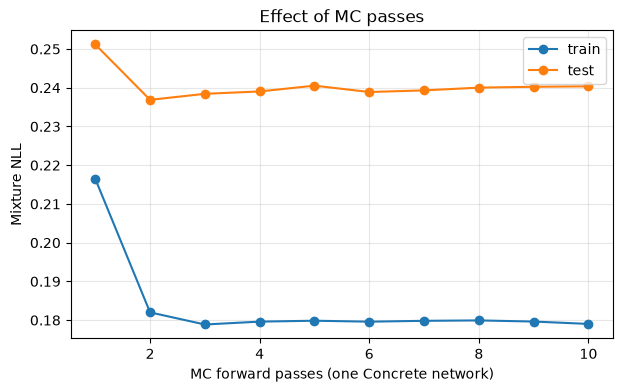
\includegraphics[width=\linewidth]{figure_06.png}
  \caption{Sensitivity of Concrete Dropout test metrics to the number of
  stochastic forward passes.}
  \label{fig:mc}
\end{figure}

\section{Conclusion}
For the synthetic problem, standard deep ensembles provide the best
point-prediction and NLL results with relatively narrow intervals, while
Concrete Dropout yields more conservative and better-covered intervals.
On diabetes, Concrete Dropout is competitive or slightly better on the
reported split, but with wider uncertainty.  The practical choice therefore
depends on whether the priority is computationally simple accuracy or a
stronger uncertainty signal from a single learned stochastic model.

\begin{thebibliography}{9}
\bibitem{lakshminarayanan2017}
 B. Lakshminarayanan, A. Pritzel, and C. Blundell.
 Simple and scalable predictive uncertainty estimation using deep ensembles.
 \emph{NeurIPS}, 2017.
\bibitem{gal2017concrete}
 Y. Gal, J. Hron, and A. Kendall.
 Concrete dropout.
 \emph{NeurIPS}, 2017.
\bibitem{gal2016}
 Y. Gal and Z. Ghahramani.
 Dropout as a Bayesian approximation: Representing model uncertainty in deep
 learning.
 \emph{ICML}, 2016.
\end{thebibliography}

\end{document}
